\documentclass[IN,english]{tumbook}
\usepackage{tabularx}
%\usepackage[utf8]{inputenc}
%\usepackage[T1]{fontenc}
%\usepackage{graphicx}
%\usepackage{amsmath}

\makeindex

% Information for the title page
\Seminar{Software Engineering for Business Applications - Master}
\Semester{SS 2015}
\title{Business Model for the Web Application \emph{Travel Diary}}
\Untertitel{}
\Themensteller{Prof. Dr. Florian Matthes}
\Autorenadresse{}
\Matrikelnummer{}
\Fachsemester{}
\Abgabetermin{13. May 2015}
\author{Chetan Basuray, Mantosh Kumar, Ulrike Niemann, Albert Steckermeier}
\date{13. May 2015}



\begin{document}

\maketitle
\newpage
\tableofcontents
\newpage

\chapter{Introduction}

In order to operate the \emph{Travel Diary} web application some form of revenue is required to establish and sustain the service. For that purpose this paper describes the business model in the structure of the business model canvas depicted in the next section.

\chapter{Business Model Canvas}


	\begin{center}
		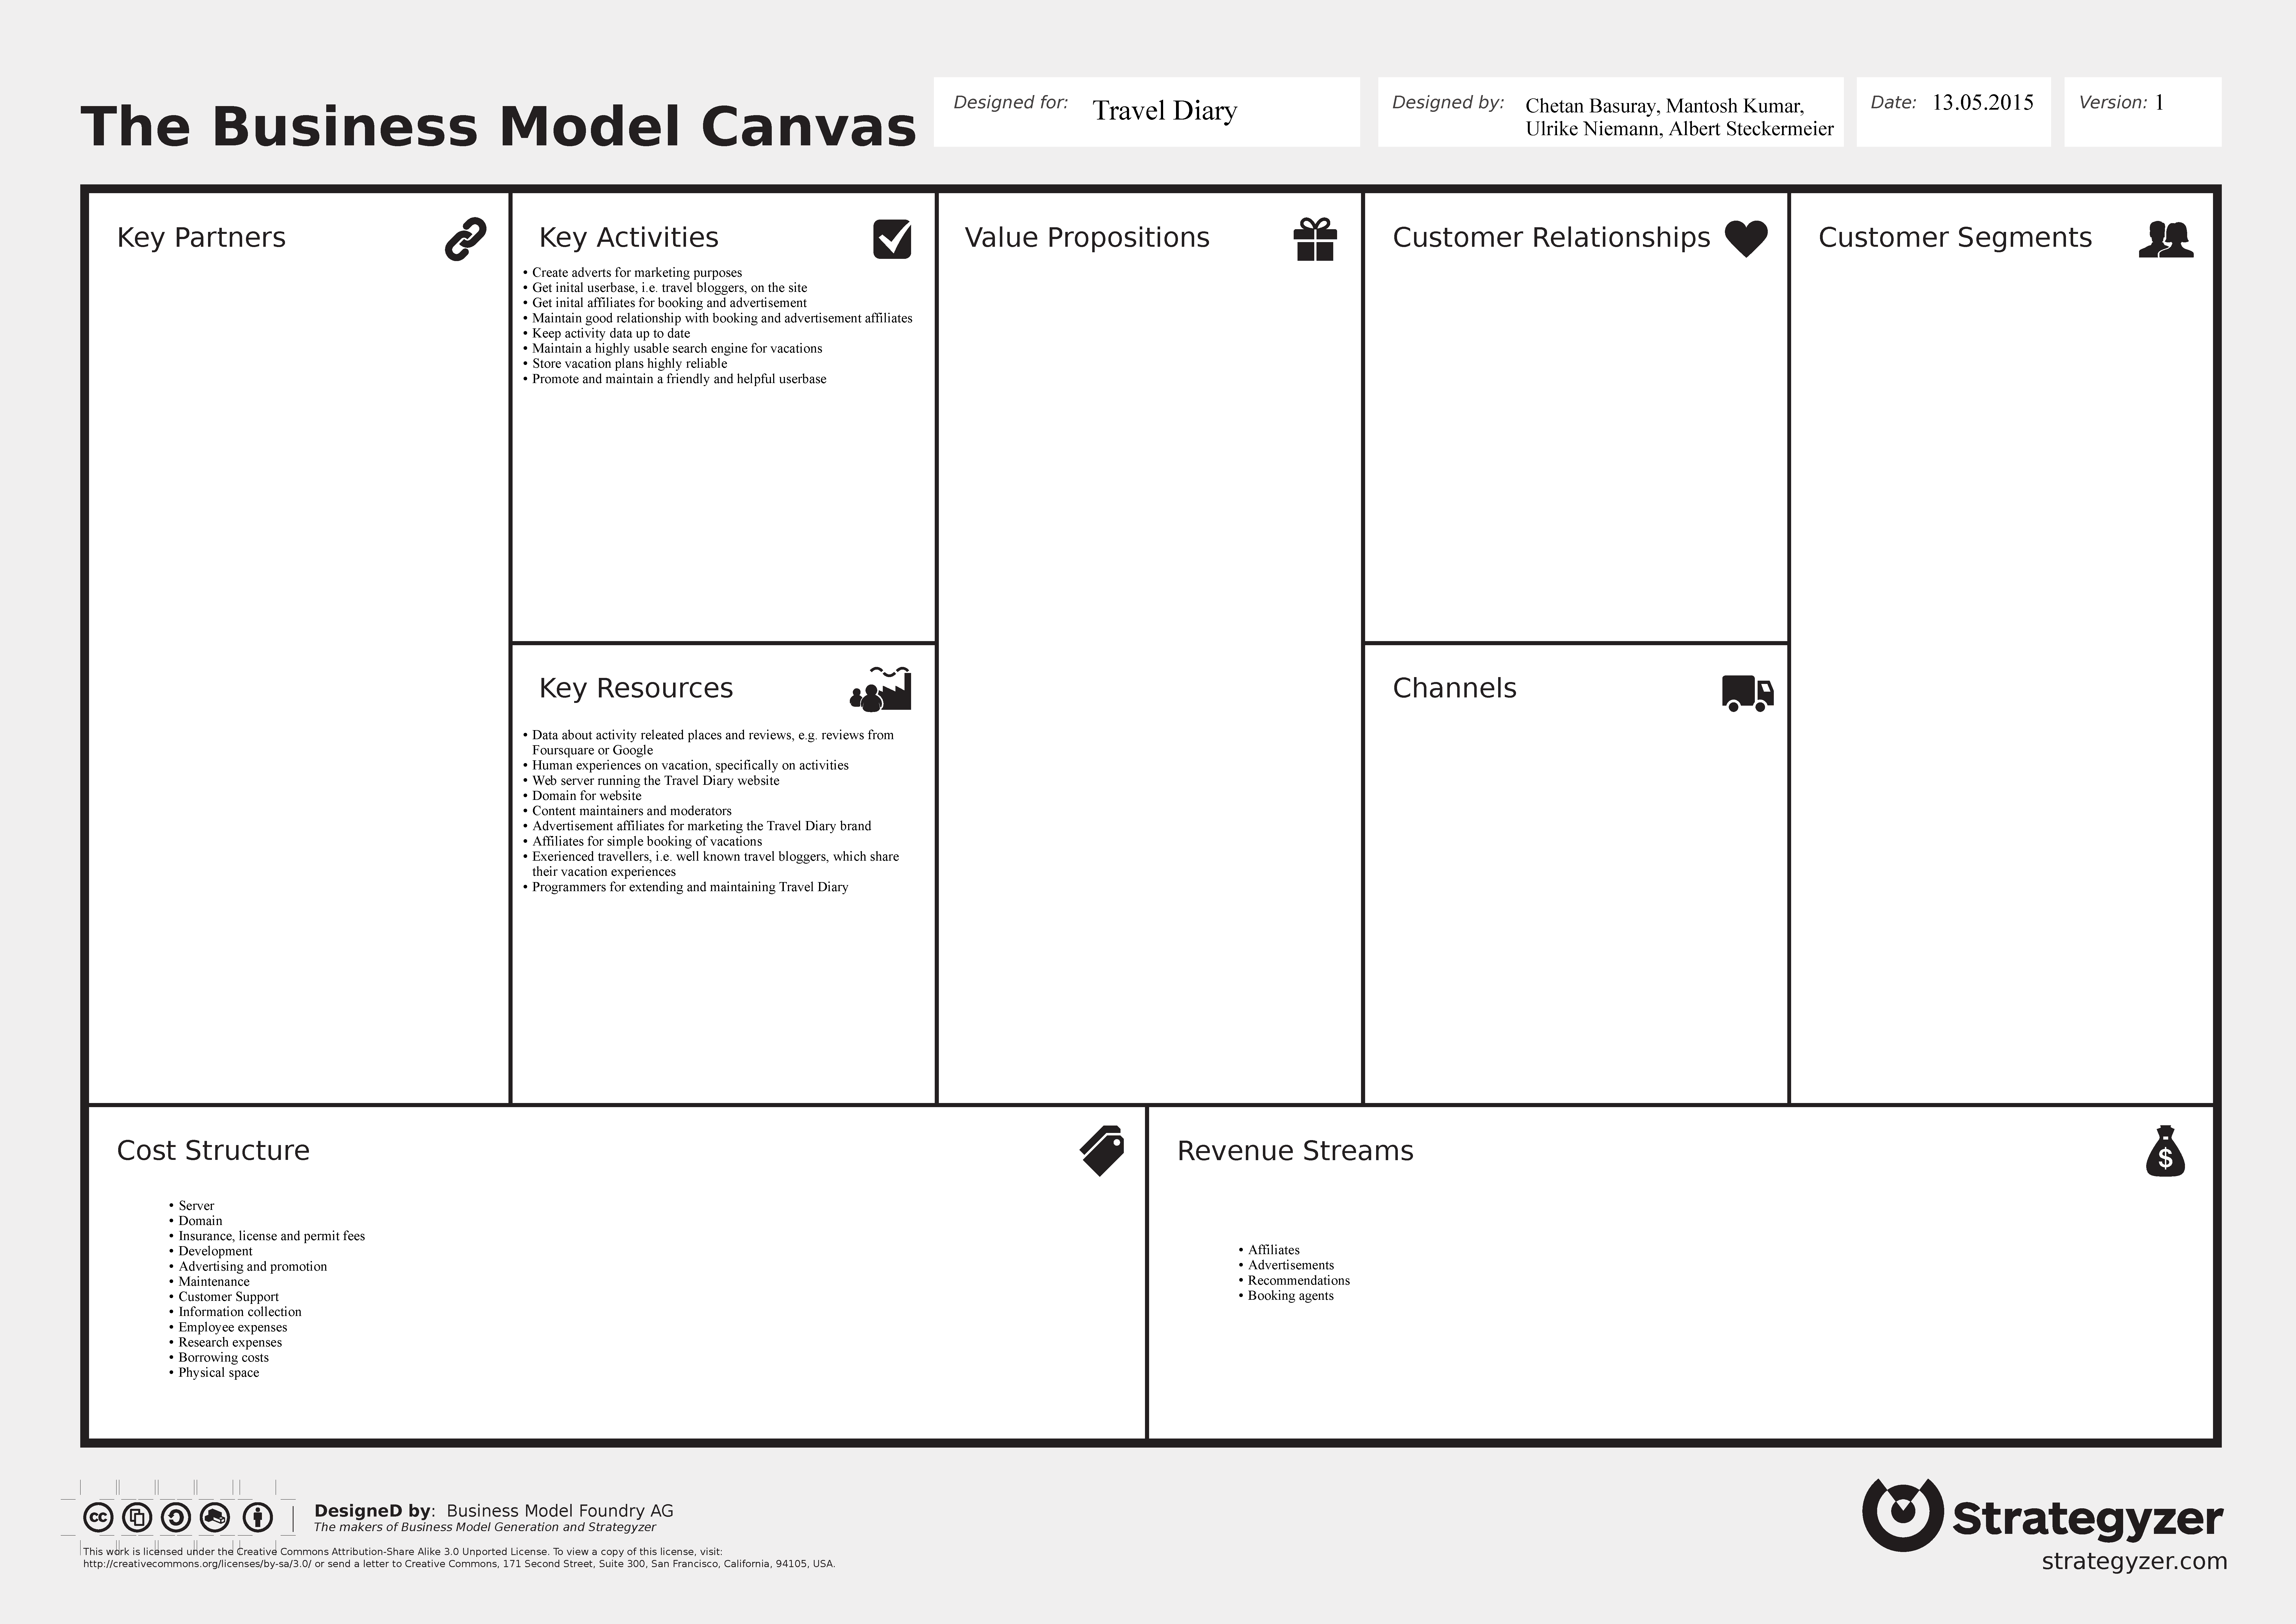
\includegraphics[scale=0.17, angle=90]{graphics/team-39-exercise-2-business-model-canvas}
	\end{center}

\chapter{Business Model}


\section{Customer Segment}

The \emph{Travel Diary} web application targets two customer segments. The first customer segment consists of people who want to plan their vacation. This includes average earners who go on a holiday at least once a year and are planning a short-term trip, i.e. two weeks long. This kind of customer wants to create a unique vacation experience with activities related to his preferences. At the same time the customer wants to do this without a hassle and with reassurance and/or insider tips from an independent, trusted source, i.e. the traveling community. The second customer segment consists of vacationists who want to share their experiences with other users, i.e. travel bloggers. They are a very important part of our concept, because they provide their experience and content on our website. The travel bloggers like to share their experiences conveniently and in an easy way. Moreover they would like to reach a large audience and receive acknowledgment for their ideas.

\section{Value Proposition}

We support vacationists in planning their vacation time and holiday activities. \emph{Travel Diary} provides a search and recommendation system for whole vacations and holiday activities related to personal preferences. For the customer it is more convenient to plan the holiday time on one site compared to browsing through many different web sites. In addition, the independent recommendations and insider tips from other travelers provide a lower risk of experiencing an unpleasant time during the vacation. Due to the preference based search and the individual composition of activities in each vacation the website offers a high level of customizability.
For travel bloggers and people who want to share their experiences the site provides a convenient way to create a public entry about a whole vacation or experience. Thus, there is no need for the customer to create and maintain an own blog or website. Moreover, the website already provides the right audience which consists of the first customer segment. However, if customers just want to record their experiences without publishing them to the whole traveling community, there is also the possibility to create a private entry in form of a diary.


\section{Customer Relationships}

Customer relationship entails all aspects of interaction that a company has with its customers. The principle benefit includes a 360-degree view of what customers and the general market want, and using this information to enhance your application.\\
\\
\emph{Travel Diary} has several categories of customer relationships.

\begin{enumerate}
\item Co-creation - The application invites customers to write reviews, share his/her trip experience and thus co-produce business and values for itself and the customers. In real sense, customers are the true champions of this application. This is \emph{Travel Diary's} primary and utmost important relationship with customers.
\item Self-service - There is no direct relationship with the customer, everything is provided to them to help themselves in FAQ section.
\item Personal assistance - This is based on human interaction. The customer can communicate with a real customer representative via chat or phone. This will obviously cost some money but is manageable as for \emph{Travel Diary} most of the purposes are served by above two relationships.
\end{enumerate}

\section{Channels}

Channels are how a company reaches its Customer Segments to deliver a Value Proposition. There is a growing interest in social procurement. To reach out to the mass \emph{Travel Diary} is planning to use web, social networks and blogging extensively. \emph{Travel Diary} is going to exhibit the experiences shared by its users as an evidence of its excellent service. Although travel agencies are its direct competitors the service plans to partner with these agencies. For customer support, there will be several segments that will address customers queries.

\section{Key Activities}

In this section the necessary key activities that keep the \emph{Travel Diary} service going will be discussed. First continuous advertising has to be implemented. The advertisement needs to be redesigned and distributed continually to fit current customer interests. Affiliate sites related to traveling will be used to advertise the \emph{Travel Diary} service. Good advertisement should get an initial user base on the site. Especially travel bloggers need to be targeted in advertisement to get enough content creators on the site. Besides advertisement, connections to affiliates for the booking of vacations have to be established. Sites like booking.com will be targeted as affiliates. When the relationships with affiliates are established they also have to cultivated. For that purpose regular feedback and personal meetings should be set up. With the affiliates the infrastructure for the service is provided but there are some maintenance activities necessary to stay competitive.\\
\\
With the help of travel bloggers as content creators a large part of the maintained activity data, i.e. related reviews and locations, should be kept up to date, but moderation of content is probably necessary. Moderation means removing deprecated user created data and reviewing user created content in terms of usefulness and sensible content. All of this should be done with the goal of creating a friendly and helpful community of travelers in mind. Consequently, the quality of data that can be searched and re-used is higher which draws more users to the service. To achieve an effective search that really yields the best possible results, the search engine has to be refined continually to achieve great search results and stand out amongst competitors. Because data loss is always a big hassle the service should also be running on a redundant platform to minimize the risk. A person for exchanging failed drives would be required if the web server is operated by the \emph{Travel Diary} team. This could however be delegated to the provider of the servers running \emph{Travel Diary}.

\section{Key Resources}

All of the activities above require some key resources to maintain the service. Affiliates for advertisement and booking will be required as can easily be seen when looking at the activities above. Also moderators, content maintainers and programmers will be needed to deal with users requests, user problems, bugs and the operation of the service. Furthermore \emph{Travel Diary} relies heavily on data about possible activities which has to be gathered or made accessible in some form. The data will be in the form of reviews which give a rough idea of the activity or place related to it. Such data could be acquired from Google Maps or Foursquare. From these sites a lot of data can be reused for the \emph{Travel Diary} service and will be enriched further by user created content. Here it is also clear that human experiences on vacation will be the enriching factor which will be one of the key data resources. A lot of experience comes from travel bloggers which will be one of the main human resources the service will require. Lastly of course the Domain as well as the web server running \emph{Travel Diary} are vital resources.

\section{Key Partners}

Key Partners for \emph{Travel Diary} are booking agencies and other specialized, search systems. For instance, a cooperation with sites like booking.com or tripadvisor.com could be established as already mentioned earlier. As these sites already have established recommendation systems for on area, i.e. hotels and accommodation, there is little overlap as \emph{Travel Diary} focuses on the planning process and holiday activities. A cooperation and linking between both sites leads to acquisition of customers for both partners. A similar cooperation is conceivable for hotels or airlines. Of course, established and experienced travel bloggers form another key partner. It would add a lot of value and high quality to the web application, if an experienced blogger adds content and recommendations. Through bloggers, there is also the possibility to attract more customers to our site when the blogger links \emph{Travel Diary} on his blog. In addition a cooperation with and linking from local tourist and/or attraction sites, i.e. a certain museums website, could also attract a lot of customers to our website.

\section{Cost Structure}

The cost structure for the business model is quite simple. We will need to have sufficient funds for a server and a domain. We would also need to have some insurance. A license and permit fees may be needed depending on the type of transactions we do and whether we need to use some proprietary software. Cost for development and maintenance of the entire project also needs to be considered and in the long run. This may also include developer fees. A big part of the expenses will be advertisements. We will need a lot of experienced writers to collect information for our site and that will be expensive. Building some sort of a customer support section, either through Facebook and emails or through phones will also need to be financed. Finally salary to be paid for the employees, either developers or otherwise will come into consideration. We will also need some expenses for researching the field we are moving into and constant research is always needed to stay ahead of competition. Finally investment will mostly come through borrowing money and there will be expenses incurred when we pay interests. Also, in the future, a demand for larger physical spaces will arise and that will need to be paid for as well.

\section{Revenue Streams}

The most important revenue streams for our website will definitely be the affiliates through which we will provide booking facilities to a customer. Directed advertisements, like those provided by google adwords, will also be an important source of revenue. Customers are willing to pay for recommendations and booking agents. By combining these two in our idea, we will be able to generate revenue since we aim to provide personalized recommendations and bookings for those.

\section{Conclusion}

To sum up, the business model is heavily based on the affiliate model. Affiliates of Travel 
Diary are sites for convenient booking of vacations like booking.com. The service will provide click through to the affiliate sites which offer simple booking mechanisms. This is the main revenue stream that keeps the service going. Furthermore Query-based Paid Placement can be used as an additional revenue source. Here a special recommended section is possible. Other businesses can pay a small fee for appearing in this section which is beneficial for them. The second revenue stream can be categorized as an advertisement model.\\
\\
We would also like to add a subscription model in future based on the number of users we have on our site. The feature would have users subscribe to our services for an annual/periodic fee and hence generate revenue. Since we will not have a large user base upfront, we do not concentrate on the subscription model for now and also do not include it in the BMC.\\
\\
\emph{Travel Diary} does not gain its primary revenue from its main audience, the travelers who visit its website. Instead, it generates revenues from business owners such as hotels, restaurants, attractions, flight companies, rental agents.\emph{Travel Diary} plans to use social media marketing such as Twitter and Facebook to let your audience know about special deals. It can use video marketing on YouTube to promote specific destinations or products and can include contextual advertising on web pages from one of the advertising networks like Google or Adbrite. The biggest advantage \emph{Travel Diary} aims to acquire is the sheer amount of reviews, recommendations and information provided by its users which could accumulate into a database whereby it will be readily accessible on the internet.\\
\\
\emph{Travel Diary} value proposition is in its wide offerings of authentic travel reviews posted by genuine travelers, who in contrast, paint a clearer picture of what is in offer as compared to purely commercially driven establishments like travel agencies. It provides a platform for travelers and consumers to interact with each other on a global scale to share their travel experiences, creating a sense of community. It creates and offers itself as a massive library of resource for travel, where consumers can find almost anything they are looking for. It is going to rely heavily on user reviews supplying fresh authentic content.

\chapter{Contribution}

\begin{table}[h]
	\begin{tabularx}{\textwidth}{|>{\setlength\hsize{\hsize}\setlength\linewidth{\hsize}}X|>{\setlength\hsize{\hsize}\setlength\linewidth{\hsize}}X|}
		\hline
		\multicolumn{1}{|c|}{Contributor} & \multicolumn{1}{|c|}{Contribution} \\
		\hline
		Chetan Basuray & 
		\begin{itemize}
			\item Wrote Cost Structure
			\item Wrote Revenue Streams
			\item Wrote Part of the Conclusion section
		\end{itemize} \\
		\hline
		Mantosh Kumar & 
		\begin{itemize}
			\item Wrote Channels
			\item Wrote Customer Relationship
		\end{itemize} \\
		\hline
		Ulrike Niemann & 
		\begin{itemize}
			\item Wrote Key Partners
			\item Wrote Value Propositions
			\item Wrote Customer Segment
		\end{itemize} \\
		\hline
		Albert Steckermeier  & 
		\begin{itemize}
			\item Wrote Introduction
			\item Wrote Key Activities
			\item Wrote Key Resources
			\item Wrote Part of the Conclusion section
		\end{itemize}
		\\
		\hline
	\end{tabularx}
	\label{tab:contribution}
	\caption{Individual contribution of the team members to this paper.}
\end{table}
\end{document}